% ---------------------------------------------------------------------------------------------------
\section{Feature engineering}
\label{section_feature_engineering}
% ---------------------------------------------------------------------------------------------------
\subsection{Categorical attributes to binary attributes}

% ---------------------------------------------------------------------------------------------------
\subsubsection{'ever\_married' and 'residence\_type'}
Two attributes ('ever\_married' and 'residence\_type') have two and only two alternative values and 
can be represented using a boolean attribute.\\

% ---------------------------------------------------------------------------------------------------
\subsubsection{'gender'}
The attribute 'gender' can be represented as a boolean attribute however, one entry for 
'gender' in the dataset is 'Other'. The values for this entry are presented in figure 
\ref{figure_gender_other}. Because its 'stroke' value is in the over-represented category, this entry 
is discarded.\\

\begin{figure}[H]
\centering
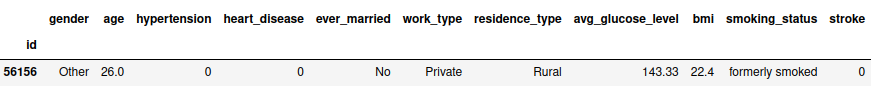
\includegraphics[scale=0.5]{figures/dataset_gender_other.png}
\caption{Entry of the database with a 'gender' value of 'Other'.}
\label{figure_gender_other}
\end{figure}

% ---------------------------------------------------------------------------------------------------
\subsubsection{'work\_type'}
Because the values of the attribute 'work\_type' (\textit{i.e.} 'Private', Govt\_job', 
'Never\_worked', 'children' and 'Self-employed') are independant and unrelated, new attributes are 
created for each of the possible value. These new attribute are numerical, binary attributes. 
 
% ---------------------------------------------------------------------------------------------------
\subsubsection{'smoking\_status'}
The attribute 'smoking\_status' has four possible values : 'unknown', 'never', 'formerly' and 
'smokes'. In order to convert this categorical attribute to numerics, two options arise. The first 
option is ordinal encoding, by associating each value to a number (\textit{e.g.} unknown 
$\rightarrow$ nan ; never $\rightarrow$ 1 ; formerly $\rightarrow$2 ; smokes $\rightarrow$ 3). The 
second option is vector encoding, by creating new attributes for each possible value.\\

Trying ordinal encoding, the correlation matrix is computed for the whole dataset and presented in 
figure \ref{figure_Xcorr_ordinal}. No strong correlation is observed between the attribute 
'smoking\_status' and the other attributes.

\begin{figure}[H]
\centering
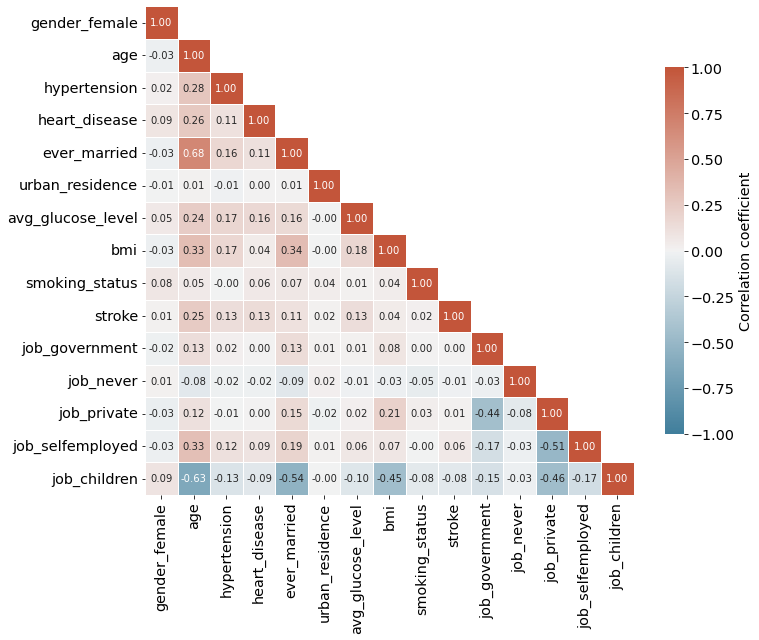
\includegraphics[scale=0.5]{../figures/correlationMatrix_smokingOrdinalEncoding.png}
\caption{Correlation matrix for ordinal encoding of 'smoking\_status' attribute.}
\label{figure_Xcorr_ordinal}
\end{figure}

Figure \ref{figure_Xcorr_vector} presents the correlation matrix for the 'smoking\_status' encoded 
with the vector encoding technique. Some relatively strong correlation appear between the new 
attributes and 'age' or 'bmi' for example as well as correlation between the new attribute 
themselves. 

\begin{figure}[H]
\centering
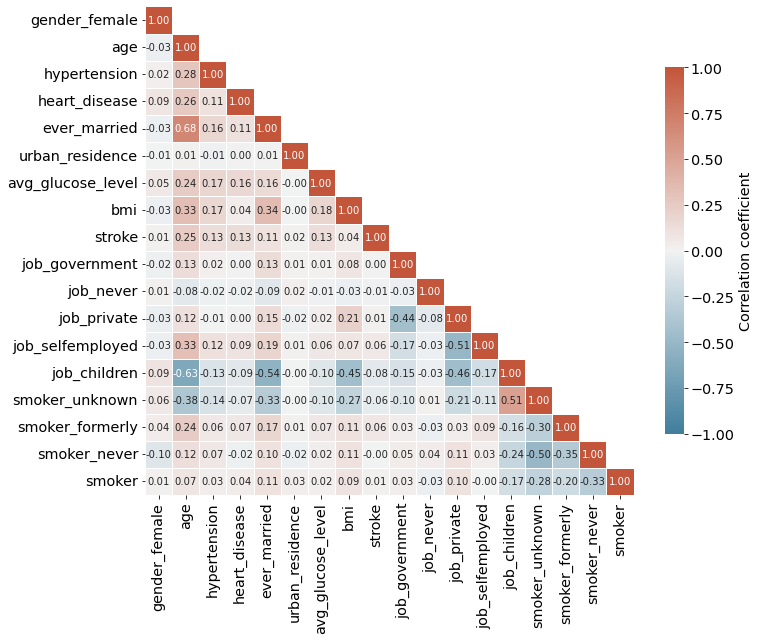
\includegraphics[scale=0.5]{../figures/correlationMatrix_smokingVectorEncoding.png}
\caption{Correlation matrix for vector encoding of 'smoking\_status' attribute.}
\label{figure_Xcorr_vector}
\end{figure}

Because the dataset and the number of attribute are not large, vector encoding is retained. Moreover, 
this encoding brings the advantage of reducint biases in the data.\\ 

The attribute 'smoker\_unknown' has $1544$ entries which correspond to the equivalent number of 
missing values. Further analysis would be necessary to assign values to the missing values however, 
considering the small correlation between this attribute and the 'stroke' attribute, 
'smoker\_unknown' is left like so in the dataset.


% ---------------------------------------------------------------------------------------------------
\subsubsection{Summary of attribute changes}
Modified attributes are summarized in table \ref{table_new_attributes}.

\begin{table}[H]\begin{tabular}{|lllc|}
\hline
\textbf{Old attribute name} & \textbf{New attribute name} & \textbf{Old values} & \textbf{New values} \\ \hline \hline
- ever\_married   & - ever\_married     & - No/Yes                & 0/1 \\ \hline
- residence\_type & - urban\_residence  & - urban/rural           & 0/1 \\ \hline
- gender          & - gender\_female    & - Male/Female           & 0/1 \\ \hline
- work\_type      & - job\_private      & - Private/Govt\_job/    & 0/1 \\
                  & - job\_government   & Never\_worked/children/ & 0/1 \\
                  & - job\_never        & Self-employed           & 0/1 \\
                  & - job\_children     &                         & 0/1 \\
                  & - job\_selfemployed &                         & 0/1 \\ \hline
- smoking\_status & - smoker\_unknown   & unkown/never/           & 0/1 \\
                  & - smoker\_never     & formerly/smokes         & 0/1 \\
                  & - smoker\_formerly  &                         & 0/1 \\
                  & - smoker            &                         & 0/1 \\ \hline
\end{tabular}
\caption{Categorical attributes transformed to binary attributes.}
\label{table_new_attributes}
\end{table}

% ---------------------------------------------------------------------------------------------------
% ---------------------------------------------------------------------------------------------------
\subsection{Missing values in the 'bmi' attribute}
Figure \ref{large_bmi} shows two unrealistic values of 'bmi' (body mass index greater than 90). 
Because the values of 'stroke' for these two entries is 0 which is over-represented, the two entries 
are removed from the dataset.\\

'bmi' attribute contains 201 missing values. A commun technique to fill the missing values is to 
assign each missing value with the average of the attribute over the dataset. In order to have a more 
accurate estimation of the missing values, 'bmi' values are compared to other numerical attributes 
with which the correlation is high. The 'age' attribute is a good candidate with a correlation 
coefficient of 0.33 (figure \ref{figure_Xcorr_vector}). The attribute 'job\_children' would have 
been a better candidate with the highest correlation coefficient (0.48) however, its boolean encoding 
makes the operation difficult and not accurate. See figure \ref{figure_age_bmi} for the distribution 
of the attributes 'age' and 'bmi'.   

\begin{figure}[H]
\centering
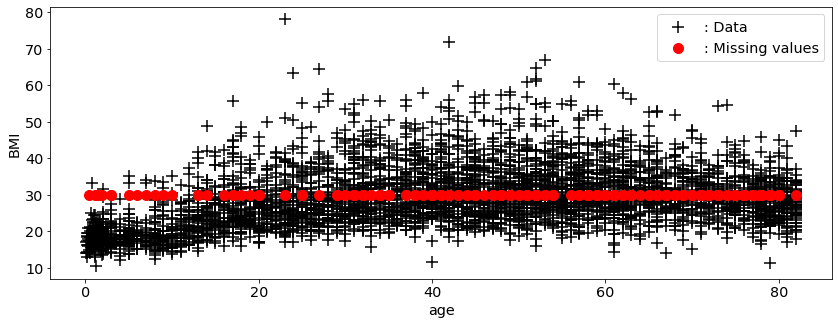
\includegraphics[scale=0.5]{../figures/plot_age_bmi_missing.png}
\caption{Distribution of the 'age' and 'bmi' attributes in black. Missing values of bmi are represented in red with a value of bmi of 30 for visual representation only.}
\label{figure_age_bmi}
\end{figure}

Thanks to the discrete values of 'age' (values of 'age' are floats when lower than 2 and integers 
when greater or equal to 2), an average value of 'bmi' is computed for each distinct 'age' value. 
See figure \ref{figure_age_bmi_replaced} for estimated values of 'bmi'. 

\begin{figure}[H]
\centering
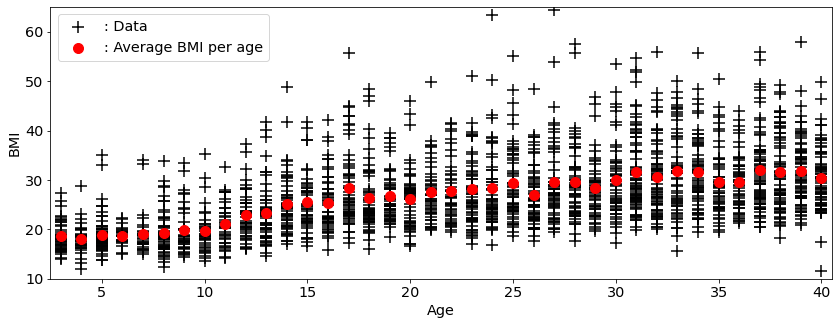
\includegraphics[scale=0.5]{../figures/plot_age_bmi_replaced.png}
\caption{Distribution of the age and bmi (black) and average BMI over age to replace the missing values of bmi (red). Zoom between age 2 and 40 to better appreciate the variation in the data.}
\label{figure_age_bmi_replaced}
\end{figure}

% ---------------------------------------------------------------------------------------------------
\subsection{Ineffective attributes}
Figure \ref{figure_Xcorr_vector} shows that there is no correlation between 'urban\_residence' and 
any other attributes. This attribute is removed from the dataset.\\

The attributes 'job\_never' and 'gender\_female' show very small correlation with other attributes. 
Their relevance might be discussed. Regarding the small size of the dataset, they are kept in this 
study.

% ---------------------------------------------------------------------------------------------------
\subsection{Bounds of the numerical attributes}
All the attributes of the dataset are numerical. All except three are boolean attributes and are in 
a the range: 'age' $\in [0.08~;~82.0]$, 'bmi' $\in [10.3~;~78.0]$ and 'avg\_glucose\_level 
$\in [106.16~;~271.7]$.

The values of these attributes are modified to be in the range $[0;1]$. We thus obtain a more uniform 
dataset.\\

Figure \ref{figure_describe_final} presents statistics of the final dataset. 

\begin{figure}[H]
\centering
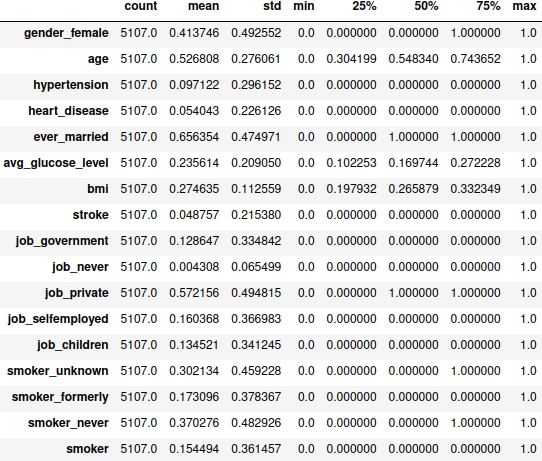
\includegraphics[scale=0.6]{figures/dataset_describe_final.png}
\caption{Statistics on dataset after feature engineering.}
\label{figure_describe_final}
\end{figure}

